
\documentclass[a4j, 10pt, uplatex]{jsarticle}
\usepackage{layout, url, resume}
\usepackage[dvipdfmx]{graphicx}
\pagestyle{empty}

\begin{document}
%\layout

\title{2016年 秋 村井研 TERM最終\\
MTA-STS : SMTP MTA Strict Transport Security
\\を用い暗号化された電子メール通信経路の確立とその実装}

% 和文著者名
\author{
    尾崎周也 (shuya) \thanks{慶應義塾大学 総合政策学部}
    \\shuya@sfc.wide.ad.jp
    \and
    親 中島博敬 (nunnun) \thanks{慶應義塾大学 政策・メディア研究科}
    \\nunnun@sfc.wide.ad.jp
}


% 和文概要
\begin{abstract}
\\
本研究はSMTPにおけるクライアント-MTA間の通信において中間者攻撃の脆弱性が存在する問題に着目し, IETF UTA Working Groupで審議中のMTA STS(SMTP MTA Strict Transport Security)\cite{draft}をJavaScriptにて実装した. 本研究はMTA-STSのポリシーでメールを送信を認証する初めての実装物である.
\end{abstract}

\maketitle
\thispagestyle{empty}

\section{背景}

SMTPはWWW以前から使用されているメール配送プロトコルの標準技術だ. SMTPは当初の仕様から今日まで改善が続けられており現在も使用されている. 電子メールは配送されるまでに1つまたは複数のMTAを経由して配送されるが, その通信経路は必ずしも暗号化されていない問題がある. [図1]
\begin{figure}[htbp]
 \begin{center}
      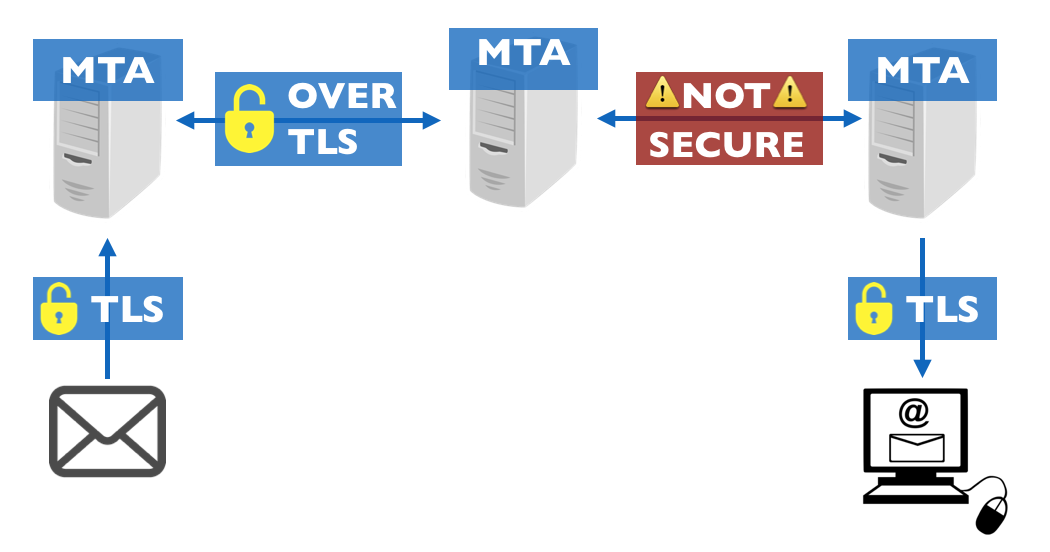
\includegraphics[width=7cm]{figure1.png}
      \caption{電子メールの配送経路}
    \end{center}
\end{figure}

STARTTLS拡張で通信経路の暗号化は行われるが, 日和見暗号化であるため能動的な攻撃を防ぐことは難しい.つまり中間者攻撃には脆弱である. ここに2つの攻撃例を示す.

\begin{itemize}
\item POODLE攻撃 
\item DNS Poisoning
\end{itemize}

\subsection{POODLE攻撃}
POODLE攻撃とは暗号化された通信から脆弱性をつき情報を盗み出す攻撃だ.現在はトランスポート層における通信秘匿技術としてTLS1.2の使用が推奨されておりほとんどのサーバやブラウザはTLS1.2に対応している. しかし全てのサーバ, ブラウザが対応しているとは限らない.そのため互換性を確保するために古い暗号方式での通信リクエストを受ける場合がある. その際, SSL3.0のようなセキュリティホールが既知化したプロトルで通信をすることが可能となる.このプロトコルのダウングレードを悪用して中間者攻撃を行うのがPOODLE攻撃である.

\subsection{DNS Poisoning}
DNS Poisoningも考えられる.DNS応答が偽造・改竄されているサーバに接続した場合, ユーザは意図しない接続先に誘導される. DNSSECで正当性が証明されない限りそのサーバが意図したものかユーザは判断することができない.

\section{研究目的}

以上から本研究では中間者攻撃に脆弱であるSMTPの現状を問題とし, SMTP-STSによるセキュアなMTA間通信を実現することを目的にする.


\section{関連技術}


\subsection{HTTP Strict Transport Security}
HSTSはWebサーバがブラウザに対して現在のアクセス以降はHTTPではなくHTTPSでの接続を強制するセキュリティ機構である. SMTP-STSの考えはこれに基づく.

\subsection{DNS-based Authentication of Named Entities(DANE)}
DANEはドメイン(DNS)とそれに証明書を発行する証明局との紐付けを明確化するセキュリティ機構だ. DANEによってサーバの応答の正当性を担保することができる.

\section{提案手法}

本研究では上記の問題を解決するためにMTA-STSを実装する.MTA-STSはSMTPの中間者攻撃への脆弱性から検討されている新しいセキュリティ機構であり, IETF UTA Working Groupで審議中だ. \cite{draft} MTA-STSの技術的特徴は2点に集約される.

\begin{itemize}
\item STARTTLSでの通信を強制する.
\item 通信経路が暗号化されていなかった場合は報告する, またはメールの受け取りを拒否する.
\end{itemize}

\section{実装}

実装はインターネットドラフトで定義されているもののうち, 接続の検証部分を実装した. 本実装はWebPKIの取得とDNSからのMTA-STSレコードの取得, 認証に用いられるSSL証明書の検証を行う.

実装環境としてはOSはCentOS6.7を使用し, 実装言語はJavaScript, クロスプラットフォームはNode.js, MTAはEximを利用した.システムの構成は次の通りである。

\begin{figure}[htbp]
 \begin{center}
      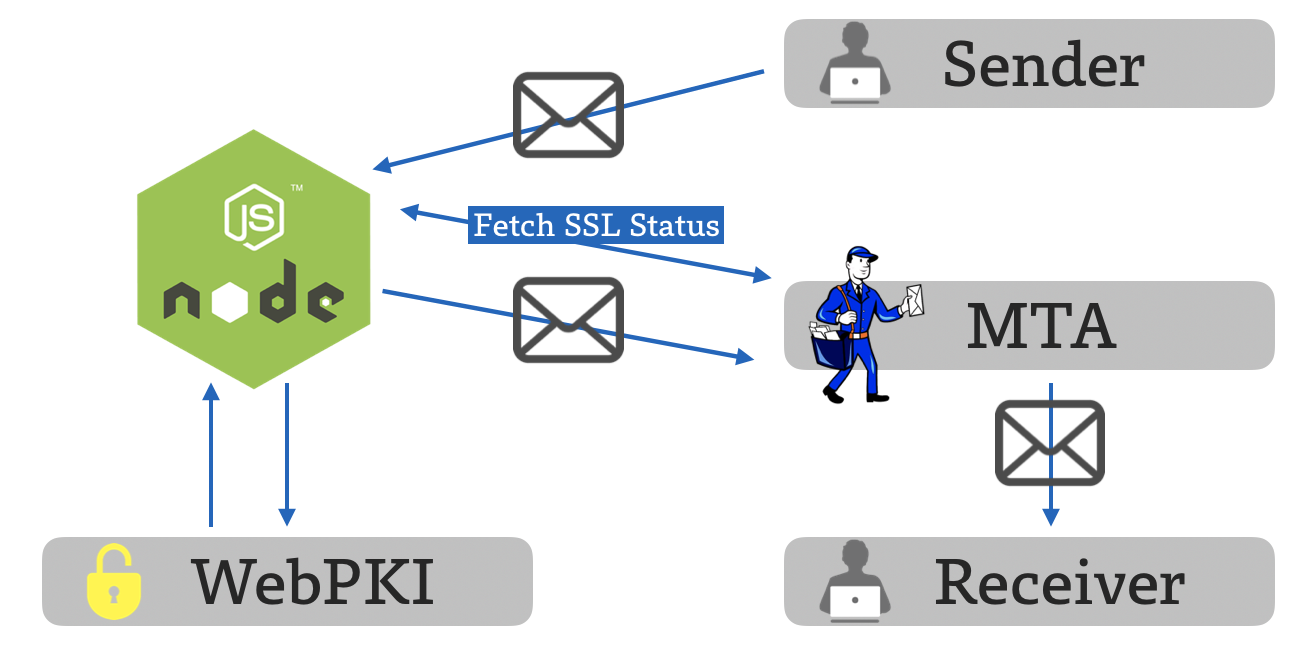
\includegraphics[width=7cm]{system.png}
      \caption{システム構成図}
    \end{center}
\end{figure}

\section{評価}

実際に本実装を使用しメールの送信を行い, 認証が正しく行われるかを検証した. MTA-STSポリシーを保持しかつ運用されているMTAにはメールが送信でき, ポリシーを持たないMTAにはメールが送信できないことを確認した.

\section{まとめ}

本研究ではMTA-STSの認証の検証結果をMTAに渡す実装を行った. 実装の過程の中で実運用されているメールサーバの多くはMTA-STSをサポートしていないこと, 今回のサーベイの中でサポートが確認できた全てのサーバが"report"モードでの運用がなされていることがわかった.



\begin{thebibliography}{9}
\bibitem{draft}
D. Margolis et al,  “SMTP Strict Transport Security”,  Internet Draft,  March 2016.\\
\url{https://tools.ietf.org/html/draft-margolis-smtp-sts-01}

\bibitem{SMTP}
A. Malatras etal,  “Technical Recommendations for Improving Security of Email Communications”,  MIPRO 2016/ISS

\bibitem{ueno}
上野宣. (2005) 『今夜わかるメールプロトコル』翔泳社.

\end{thebibliography}

\end{document}
% end of file
